\documentclass["WS\space 16-17\space -\space LaTeX-Kurs\space -\space Praesentation\space -\space 3.tex"]{subfiles}

\begin{document}

\section{Literaturverweise}
\begin{frame}[c]
	\begin{center}
		\LARGE \textbf{Literaturverweise}
	\end{center}
\end{frame}
%%-----------------------------------------------------------------------------------------------%
%%------------------------------------------SUBSECTION-------------------------------------------%
%%-----------------------------------------------------------------------------------------------%
\subsection{Grundlagen}
\begin{frame}[c]
	\begin{center}
		\large Grundlagen
	\end{center}
\end{frame}
%-----------------------------------------------------------------------------------%
%---------------------------------------Einleitung----------------------------------%
%-----------------------------------------------------------------------------------%
\begin{frame}[c]

  \begin{columns}[c]
    \column{0.5\textwidth}
    \begin{block}{How to:}
      \begin{itemize}
      \item Es gibt keinen 100\%ig einheitlichen Stil! Aber grob:
      \item Bezeichner im Text
      \item Verzeichnis im Anhang
      \end{itemize}
    \end{block}
    
    \column{0.5\textwidth}
    \begin{figure}
      \centering
      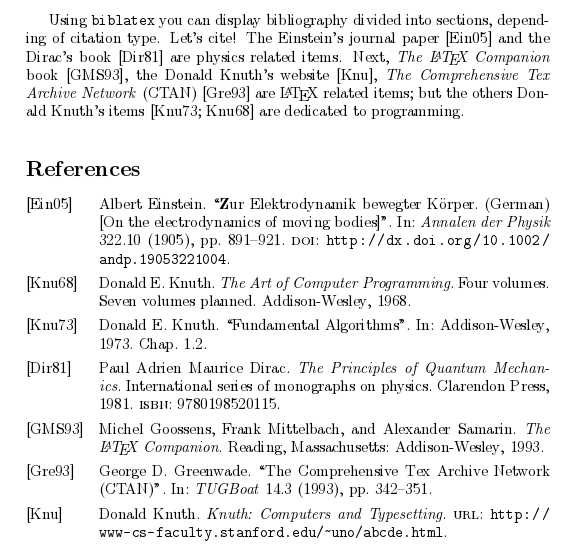
\includegraphics[width=\linewidth]{img/BiblatexExample.png}
      \label{fig:BiblatexExample}
    \end{figure}
    $^[$\footnotemark$^]$ %caption prints ``Abbildung 1:'' which is annoying
  \end{columns}
  \footnotetext{Entnommen aus \cite{ShLaTeX}}
  
\end{frame}


\subsection{\hologo{BibTeX}}


\begin{frame}[c,fragile]

  \begin{center}
    \resizebox{0.2\textwidth}{!}{\hologo{BibTeX}}
  \end{center}
  
  \begin{columns}[c]
    \column{0.5\textwidth}
    \begin{center}
      \begin{block}{Anforderung}
        \begin{itemize}
        \item Konsistent
        \item Effizient
        \item Automatisiert
        \end{itemize}
      \end{block}
    \end{center}

    \column{0.5\textwidth}
    \begin{center}
      \begin{block}{Realisierung}
        \begin{itemize}
        \item Schlüsselwort - Formalismus
        \item Bekannt von \lstinline[basicstyle=\ttfamily\normalsize]|\label|-\lstinline[basicstyle=\ttfamily\normalsize]|\ref|
        \end{itemize}
      \end{block}
    \end{center}
  \end{columns}

  \begin{center}
    \begin{tabular}{r | l}
      \toprule
      \lstinline[basicstyle=\ttfamily\normalsize]|\label|-\lstinline[basicstyle=\ttfamily\normalsize]|\ref| - Formalismus & \hologo{BibTeX} - Formalismus \\
      \midrule
      \only<1>{\texttt{\textbackslash \color{green!70!black}{label}\color{black}{\{}}\textit{\small{<label-keyword>}}\texttt{\}}}%
      \only<2>{\textit{\small{<Quellcode-Dateiname>}}\texttt{\color{teal}{.aux}}}
      & \textit{\small{<Bibliotheks-Dateiname>}}\texttt{\color{teal}{.bib}} \\
      \texttt{\textbackslash \color{green!70!black}ref\color{black}\{}\textit{\small{<label-keyword>}}\texttt{\}} & \texttt{\textbackslash \color{green!70!black}cite\color{black}\{}\textit{\small{<bib-keyword>}}\texttt{\}}\\
      \bottomrule
    \end{tabular}
    \note[item]<1->{Quelle des keywords ist \lstinline|\label| bzw \texttt{.bib}-Datei.}
    \note[item]<1->{Lüften das Geheimnis der \texttt{\color{teal}{.aux}}-Datei: Sie ist die eigentliche Quelle, hier notiert sich \LaTeX, was es beim nächsten mal kompilieren wissen muss.}
  \end{center}
  
\end{frame}

%-----------------------------------------------------------------------------------%
%---------------------------------------FRAME---------------------------------------%
%-----------------------------------------------------------------------------------%
\begin{frame}[fragile]
	\begin{Aufgabe}
		Füge in die Bildunterschrift zur Löwenjagd eine Referenz auf \textrm{bear} ein und schreibe in das optionale Argument des \lstinline[basicstyle=\normalfont\normalsize]|\cite|-Befehls den Text \textrm{\qquote{bearbeitet}}:
	\end{Aufgabe}
	\begin{outputbox}
		\vspace{-0.3cm}
		\begin{center}
			\textbf{Abbildung 1} - \textit{Vergleich verschiedener Dienste bei der Löwenjagd. [1, bearbeitet]}
		\end{center}
		\vspace{-0.3cm}
	\end{outputbox}
	\btVFill\Befehle
	\begin{center}
		\begin{tabular}{ll}
			\toprule
			\LaTeX\ Befehl							&	Funktion					\\ \midrule
			\lstinline|\cite[]{}|					&	Zitierbefehl\\
			\lstinline|\printbibliography|			&	Erstellen des Literaturverzeichnis\\
			\lstinline|\citeauthor{}|				&	Zitieren des Autors \\
			\lstinline|\citeyear{}|					&	Zitieren des Jahrs \\
			\lstinline|\citetitle{}|				&	Zitieren des Titels \\
			\lstinline|\psq|, \lstinline|\psqq|		&	\texttt{f} und \texttt{ff} \\
			\bottomrule
		\end{tabular}
	\end{center}
	\vspace{0.1cm}
\end{frame}


\begin{frame}[fragile]
	\begin{onlyenv}<1,2>
		\Ausgabe
		\begin{outputbox}
			Dieser Abschnitt ist an \cite{Petard1938} angelehnt.
		\end{outputbox}
		\linebreakrule
		\begin{outputbox}
			\makebox[1cm]{$[1]$} H. P\'{e}tard. \qquote{Ein Beitrag zur Mathematischen Theorie der Großwildjagd}.\\
			\makebox[1cm]{} In: \textit{American Mathematical Monthly} 54 (1938), S. 466.
		\end{outputbox}
	\end{onlyenv}
	\begin{onlyenv}<2>
		\Code
		\begin{lstlisting}
	Entnommen aus \cite{Petard1938}
		\end{lstlisting}
		\begin{lstlisting}
	\printbibliography
		\end{lstlisting}
	\end{onlyenv}
	\begin{onlyenv}<3,4>
		\Ausgabe
		\begin{outputbox}
			Dieser Abschnitt ist an \cite[20\psqq]{Petard1938} angelehnt.
		\end{outputbox}
		\linebreakrule
		\begin{outputbox}
			\makebox[1cm]{$[1]$} H. P\'{e}tard. \qquote{Ein Beitrag zur Mathematischen Theorie der Großwildjagd}.\\
			\makebox[1cm]{} In: \textit{American Mathematical Monthly} 54 (1938), S. 466.
		\end{outputbox}
	\end{onlyenv}
	\begin{onlyenv}<4>
		\Code
		\begin{lstlisting}
Entnommen aus \cite[20\psqq]{Petard1938}
		\end{lstlisting}
		\begin{lstlisting}
\printbibliography
		\end{lstlisting}
	\end{onlyenv}
\end{frame}
%-----------------------------------------------------------------------------------%
%---------------------------------------FRAME---------------------------------------%
%-----------------------------------------------------------------------------------%
\begin{frame}[fragile]
	\begin{Aufgabe}
		Füge im ersten Abschnitt \qquote{Vergleich der Körpereigenschaften} Zitate zu den beiden Quellen \textrm{WALowe} und \textrm{WAMensch} an den Text an:
		\begin{outputbox}
			Wenn nicht anders angegeben sind die Daten in Tabelle 1 von der Wissensmaschine WolframAlpha [6], [7].
		\end{outputbox}
		und erstelle am Ende des Dokuments eine neue Seite mit dem Literaturverzeichnis.
	\end{Aufgabe}
	\btVFill\Befehle
	\begin{center}
		\begin{tabular}{ll}
			\toprule
			\LaTeX\ Befehl							&	Funktion					\\ \midrule
			\lstinline|\cite[]{}|					&	Zitierbefehl\\
			\lstinline|\printbibliography|			&	Erstellen des Literaturverzeichnis\\
			\lstinline|\citeauthor{}|				&	Zitieren des Autors \\
			\lstinline|\citeyear{}|					&	Zitieren des Jahrs \\
			\lstinline|\citetitle{}|				&	Zitieren des Titels \\
			\lstinline|\psq|, \lstinline|\psqq|		&	\texttt{f} und \texttt{ff} \\
			\bottomrule
		\end{tabular}
	\end{center}
	\vspace{0.1cm}
\end{frame}
%-----------------------------------------------------------------------------------%
%---------------------------------------FRAME---------------------------------------%
%-----------------------------------------------------------------------------------%
\begin{frame}[fragile]
	\Losung
	\begin{outputbox}
		Wenn nicht anders angegeben sind die Daten in Tabelle 1 von der Wissensmaschine WolframAlpha [6], [7].
	\end{outputbox}
	\linebreakrule\vspace{-0.3cm}
	$\cdots$
	\linebreakrule
	\begin{outputbox}
		{\LARGE \textbf{Literaturverzeichnis}}
		
		\makebox[1cm]{$[6]$} WolframAlpha. \textit{human}. 5.10.2016.\\
		\makebox[1cm]{} \texttt{url:} \lstinline|http://www.wolframalpha.com/input/?i=human.|
		
		\makebox[1cm]{$[7]$} WolframAlpha. \textit{lion}. 5.10.2016.\\
		\makebox[1cm]{} \texttt{url:} \lstinline|http://www.wolframalpha.com/input/?i=lion.|
	\end{outputbox}
	\Code
	\begin{lstlisting}
Wenn nicht anders angegeben sind die Daten in Tabelle 1 von der Wissensmaschine WolframAlpha \cite{WALowe}, \cite{WAMensch}.
...
\newpage
\printbibliography
	\end{lstlisting}
\end{frame}
%-----------------------------------------------------------------------------------%
%---------------------------------------FRAME---------------------------------------%
%-----------------------------------------------------------------------------------%
\begin{frame}[fragile]
	\begin{Aufgabe}
		Füge in die beiden letzten Einträge der Tabelle zum Grundstoffwechselumsatz in der Spalte \qquote{Löwe} eine Referenz auf \textrm{HAGRLowe} und unter \qquote{Mensch} eine Referenz auf \textrm{HAGRMensch} ein.
	\end{Aufgabe}
	\begin{outputbox}
		\begin{tabular}{rcc}
			...&&\\
			Grundstoffwechselumsatz	&	\SI{94.58 }{\kg\metre\tothe{2}\per\second\tothe{3}}	\cite{HAGRLowe}		&	\SI{82.78}{\watt}	\cite{HAGRMensch}
		\end{tabular}
	\end{outputbox}
	\btVFill\Befehle
	\begin{center}
		\begin{tabular}{ll}
			\toprule
			\LaTeX\ Befehl							&	Funktion					\\ \midrule
			\lstinline|\cite[]{}|					&	Zitierbefehl\\
			\lstinline|\printbibliography|			&	Erstellen des Literaturverzeichnis\\
			\lstinline|\citeauthor{}|				&	Zitieren des Autors \\
			\lstinline|\citeyear{}|					&	Zitieren des Jahrs \\
			\lstinline|\citetitle{}|				&	Zitieren des Titels \\
			\lstinline|\psq|, \lstinline|\psqq|		&	\texttt{f} und \texttt{ff} \\
			\bottomrule
		\end{tabular}
	\end{center}
	\vspace{0.1cm}
\end{frame}
%-----------------------------------------------------------------------------------%
%---------------------------------------FRAME---------------------------------------%
%-----------------------------------------------------------------------------------%
\begin{frame}[fragile]
	\Losung
	\begin{outputbox}
		\begin{tabular}{rcc}
			...&&\\
			Grundstoffwechselumsatz	&	\SI{94.58 }{\kg\metre\tothe{2}\per\second\tothe{3}}	\cite{HAGRLowe}		&	\SI{82.78}{\watt}	\cite{HAGRMensch}
		\end{tabular}
	\end{outputbox}
	\Code
	\begin{lstlisting}[tabsize=1]
Grundstoffwechselumsatz
& \SI{94.58}{\kg\metre\tothe{2}\per\second\tothe{3}} \cite{HAGRLowe}
& \SI{82.78}{\watt} \cite{HAGRMensch}
	\end{lstlisting}
\end{frame}
%-----------------------------------------------------------------------------------%
%---------------------------------------FRAME---------------------------------------%
%-----------------------------------------------------------------------------------%
\begin{frame}[fragile]
	\Losung
	\begin{outputbox}
		\begin{centering}
			\begin{tabular}{rcc}
				...&&\\
				Grundstoffwechselumsatz	&	\SI{94.58 }{\kg\metre\tothe{2}\per\second\tothe{3}}	\cite{HAGRLowe}		&	\SI{82.78}{\watt}	\cite{HAGRMensch}
			\end{tabular}
		\end{centering}
	\end{outputbox}
	\Code
	\begin{lstlisting}
\begin{figure}
	\centering
	\includegraphics[width=0.3\textwidth]{Bilder/LionJagd.png}
	\caption{Vergleich verschiedener Dienste bei der Löwenjagd. \cite[bearbeitet]{bear}}
	\label{fig:lionjagd}
\end{figure}
	\end{lstlisting}
\end{frame}
%%-----------------------------------------------------------------------------------------------%
%%------------------------------------------SUBSECTION-------------------------------------------%
%%-----------------------------------------------------------------------------------------------%
\subsection{Das Literaturverzeichnis}
\begin{frame}[c]
	\begin{center}
		\large Das Literaturverzeichnis
	\end{center}
\end{frame}
%-----------------------------------------------------------------------------------%
%---------------------------------------FRAME---------------------------------------%
%-----------------------------------------------------------------------------------%
\begin{frame}[fragile]
	\begin{lstlisting}
Literaturverzeichnis.bib
	\end{lstlisting}
	\begin{lstlisting}
@TYP{BEZEICHNUNG,
	FELD1	=	{},
	FELD2	=	{},
	FELD3	=	{},
	FELD4	=	{},
}
	\end{lstlisting}
	\begin{center}
		\begin{tabular}{ll}
			\toprule					
			Typen			&	erforderliche Felder						\\ \midrule
			article			&	author, title, journal, year				\\	
			book			&	author/editor, title, publisher, year		\\
			techreport		&	author, title, institution, year			\\
			\bottomrule
		\end{tabular}
	\end{center}
	\vspace{0.1cm}
\end{frame}
%-----------------------------------------------------------------------------------%
%---------------------------------------FRAME---------------------------------------%
%-----------------------------------------------------------------------------------%
\begin{frame}
	Aber damit man das nicht alles per Hand machen muss gibt es Websites wie z.B.:
	\href{http://literatur-generator.de}{\textrm{literatur-generator.de}}.
\end{frame}
\note{
- Zum Browser gehen und zeigen!\\
- bei anderen Quellen (z.B. Wiki) gibt es auch oft eine Option zum Export nach biblatex}
%-----------------------------------------------------------------------------------%
%---------------------------------------FRAME---------------------------------------%
%-----------------------------------------------------------------------------------%
\begin{frame}[fragile]
	\begin{Aufgabe}
		Öffne die Datei \qquote{Literaturverzeichnis.bib} und schau dir den Aufbau der bestehenden Einträge an.
	\end{Aufgabe}
	\begin{Aufgabe}
		Benutze nun \href{http://literatur-generator.de}{\textrm{literatur-generator.de}} um dir einen Eintrag für das Buch
		
		\hspace{0.5cm}\textrm{\qquote{Kabinett physikalischer Raritäten - Eine Anthologie zum Mit-, Nach- u. Weiterdenken}}
		
		von
		
		\hspace{0.5cm}\textrm{Robert L. Weber} und \textrm{Eric Mendoza} (\texttt{ISBN: 978-3-663-14075-7})
		
		erstellen zu lassen und füge ihn in die Datei \qquote{Literaturverzeichnis.bib} ein.
	\end{Aufgabe}
\end{frame}
%-----------------------------------------------------------------------------------%
%---------------------------------------FRAME---------------------------------------%
%-----------------------------------------------------------------------------------%
\begin{frame}[fragile]
	\Code
	\begin{lstlisting}
@BOOK{Weber2013,
	AUTHOR		= {Weber, Robert L. AND Mendoza, Eric},
	YEAR		= {2013},
	TITLE		= {Kabinett physikalischer Raritäten - Eine Anthologie zum Mit-, Nach- u. Weiterdenken},
	EDITION 	= {},
	ISBN		= {978-3-663-14075-7},
	PUBLISHER	= {Springer-Verlag},
	ADDRESS		= {Berlin Heidelberg New York},
}
	\end{lstlisting}
\end{frame}

\end{document}